\documentclass{standalone}
%convert -density 300 timing_diagram.pdf timing_diagram.png
\usepackage[usenames,dvipsnames]{xcolor}
\usepackage{tikz}
\usetikzlibrary{arrows}

\begin{document}
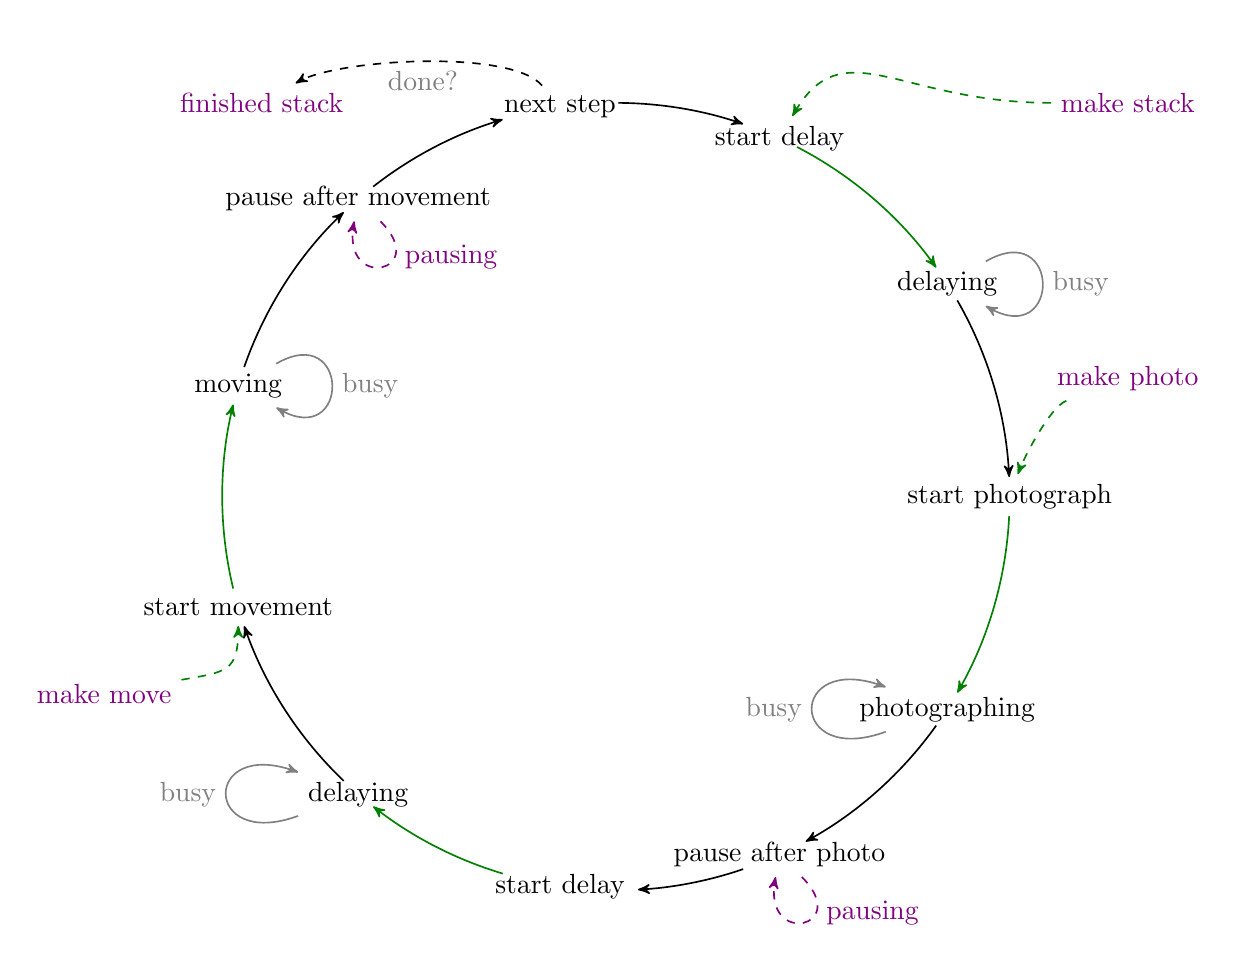
\begin{tikzpicture}[>=stealth',semithick]

    \tikzstyle{substate}=[]

    \tikzstyle{transition}=[<-]
    \tikzstyle{lambda}=[Green]
    \tikzstyle{metatransition}=[dashed] % in and out of stacking
    \tikzstyle{busyloop}=[transition, gray]
    \tikzstyle{busytext}=[gray]
    \tikzstyle{metaloop}=[dashed, Purple]
    \tikzstyle{metatext}=[Purple]
    \tikzstyle{metastate}=[Purple]

    \def \stateN {11} % number of states in the circle
    \def \stateR {5cm} % radius of the state circle.
    \def \stateRot {3} % shift by hand
    \def \margin {0.1cm};

    \newcommand\statetransition[6]{
        \draw[#4] ({360/\stateN * (#1 - 1)+#2}:\stateR) arc ({360/\stateN * (#1 - 1)+#2}:{360/\stateN * (#1)-#3}:\stateR) node[pos=0.5, #5] {#6};
    }
    %\\statetransition{pos}{lmargin}{rmargin}{linestyle}{nodestyle}{nodetext};

    % create the substates
    \node[substate] (start_delay_before_photo) at ({-360/\stateN * (1 - \stateRot)}:\stateR) {start delay};
    \node[substate] (delay_before_photo)  at ({-360/\stateN * (2 - \stateRot)}:\stateR) {delaying};
    \node[substate] (start_photo)  at ({-360/\stateN * (3 - \stateRot)}:\stateR) {start photograph};
    \node[substate] (photo_busy)  at ({-360/\stateN * (4 - \stateRot)}:\stateR) {photographing};
    \node[substate] (pause_after_photo)  at ({-360/\stateN * (5 - \stateRot)}:\stateR) {pause after photo};
    \node[substate] (start_delay_after_photo)  at ({-360/\stateN * (6 - \stateRot)}:\stateR) {start delay};
    \node[substate] (delay_after_photo)  at ({-360/\stateN * (7 - \stateRot)}:\stateR) {delaying};
    \node[substate] (start_movement)  at ({-360/\stateN * (8 - \stateRot)}:\stateR) {start movement};
    \node[substate] (movement)  at ({-360/\stateN * (9 - \stateRot)}:\stateR) {moving};
    \node[substate] (pause_after_movement)  at ({-360/\stateN * (10 - \stateRot)}:\stateR) {pause after movement};
    \node[substate] (next_step)  at ({-360/\stateN * (11 - \stateRot)}:\stateR) {next step};

    % position the 'meta' states; where the state machine has its entrypoint etc.
    \node[metastate,] (make_stack) at (6.5,5) {make stack};
    \node[metastate] (make_photo) at (6.5,1.5) {make photo};
    \node[metastate] (make_move) at (-6.5,-2.5) {make move};
    \node[metastate] (halted) at (-4.5,5) {finished stack};

    % create the state -> substate transitions.
    \draw [->, metatransition, lambda] (make_stack) to [out=180,in=60,out looseness=1.5](start_delay_before_photo);
    \draw [->, metatransition] (next_step) to [out=130,in=30,looseness=0.5] node[pos=0.5, below, busytext] {done?} (halted);
    \draw [->, metatransition, lambda] (make_photo) to [out=200,in=70,looseness=0.5] (start_photo);
    \draw [->, metatransition, lambda] (make_move) to [out=10,in=270,looseness=1.5] (start_movement);


    % create the loops of the main state machine.
    \draw [<-, busyloop] (movement) to  [out=-30,in=30,looseness=5]  node[pos=0.5, right, busytext] {busy} (movement);

    \draw [<-, busyloop] (photo_busy) to  [out=160,in=200,looseness=6]  node[pos=0.5, left, busytext] {busy} (photo_busy);

    \draw [->, busyloop] (delay_before_photo) to [out=-30,in=30,looseness=5]  node[pos=0.5, right, busytext] {busy} (delay_before_photo);
    \draw [->, busyloop] (delay_after_photo) to [out=160,in=200,looseness=6]  node[pos=0.5, left, busytext] {busy} (delay_after_photo);

    \draw [->, metaloop] (pause_after_movement) to [out=-45,in=-100,looseness=7]  node[pos=0.3, right, metatext] {pausing} (pause_after_movement);
    \draw [->, metaloop] (pause_after_photo) to [out=-45,in=-100,looseness=7]  node[pos=0.3, right, metatext] {pausing} (pause_after_photo);

    % create the arrows on the circle.
    \statetransition{1}{0.1cm}{0.1cm}{transition}{}{};
    \statetransition{2}{0.1cm}{0.1cm}{transition, lambda}{}{};
    \statetransition{3}{0.2cm}{0.3cm}{transition}{}{};
    \statetransition{4}{0.3cm}{0.1cm}{transition}{}{};
    \statetransition{5}{0.1cm}{0.1cm}{transition}{}{};
    \statetransition{6}{0.1cm}{0.1cm}{transition, lambda}{}{};
    \statetransition{7}{0.1cm}{0.1cm}{transition}{}{};
    \statetransition{8}{0.1cm}{0.3cm}{transition, lambda}{}{};
    \statetransition{9}{0.4cm}{0.2cm}{transition}{}{};
    \statetransition{10}{0.15cm}{0.1cm}{transition}{}{};
    \statetransition{11}{0.1cm}{0.1cm}{transition, lambda}{}{};
 
\end{tikzpicture}
\end{document}